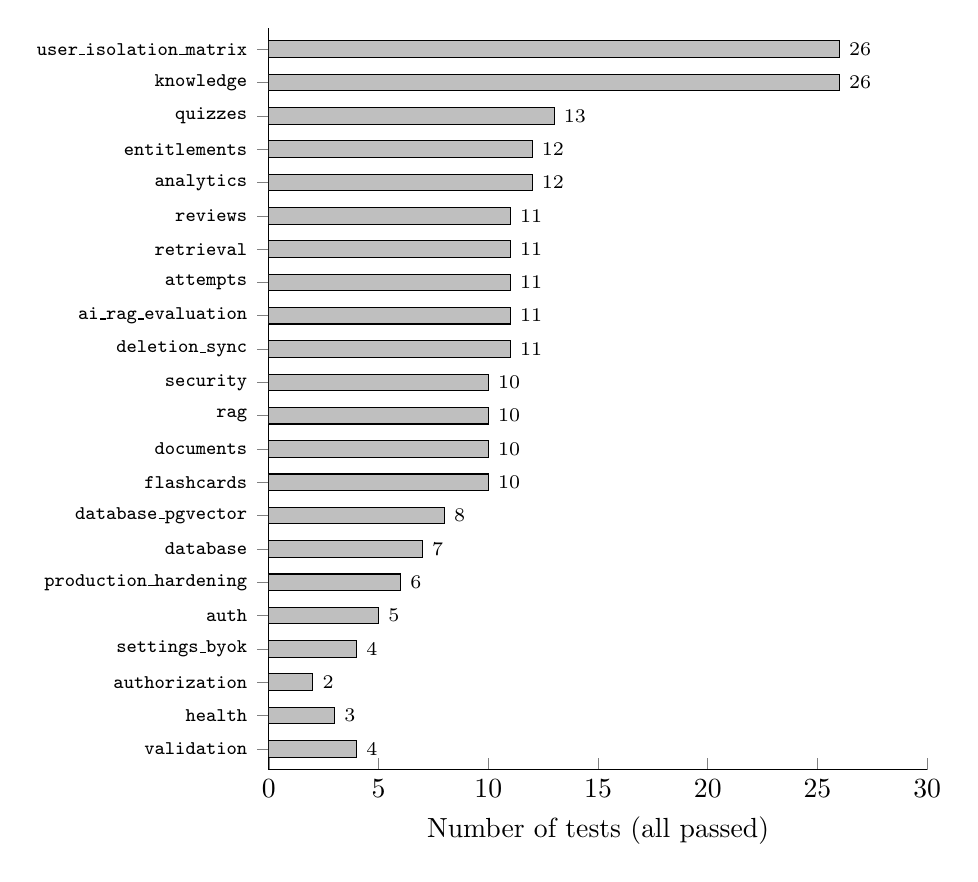
\begin{tikzpicture}
\begin{axis}[
  xbar, width=0.82\textwidth, height=11cm,
  bar width=6pt, xmin=0, xmax=30,
  xlabel={Number of tests (all passed)},
  symbolic y coords={validation,health,authorization,settings\_byok,auth,production\_hardening,database,database\_pgvector,flashcards,documents,rag,security,deletion\_sync,ai\_rag\_evaluation,attempts,retrieval,reviews,analytics,entitlements,quizzes,knowledge,user\_isolation\_matrix},
  ytick=data, y tick label style={font=\scriptsize\ttfamily},
  nodes near coords, nodes near coords style={font=\scriptsize},
  enlarge y limits=0.03, axis lines*=left]
\addplot[fill=black!25, draw=black] coordinates {(4,validation) (3,health) (2,authorization) (4,settings\_byok) (5,auth) (6,production\_hardening) (7,database) (8,database\_pgvector) (10,flashcards) (10,documents) (10,rag) (10,security) (11,deletion\_sync) (11,ai\_rag\_evaluation) (11,attempts) (11,retrieval) (11,reviews) (12,analytics) (12,entitlements) (13,quizzes) (26,knowledge) (26,user\_isolation\_matrix)};
\end{axis}
\end{tikzpicture}
